\documentclass[12pt]{standalone}
\usepackage{xcolor}
\usepackage{amssymb}

\usepackage{tikz}

\newcommand{\Cross}{$\mathbin{\tikz [solid,x=2ex,y=2ex,line width=.4ex, red] \draw (0,0) -- (1,1) (0,1) -- (1,0);}$}%

\newcommand{\Checkmark}{\LARGE $\color{green}\checkmark$}

\begin{document}

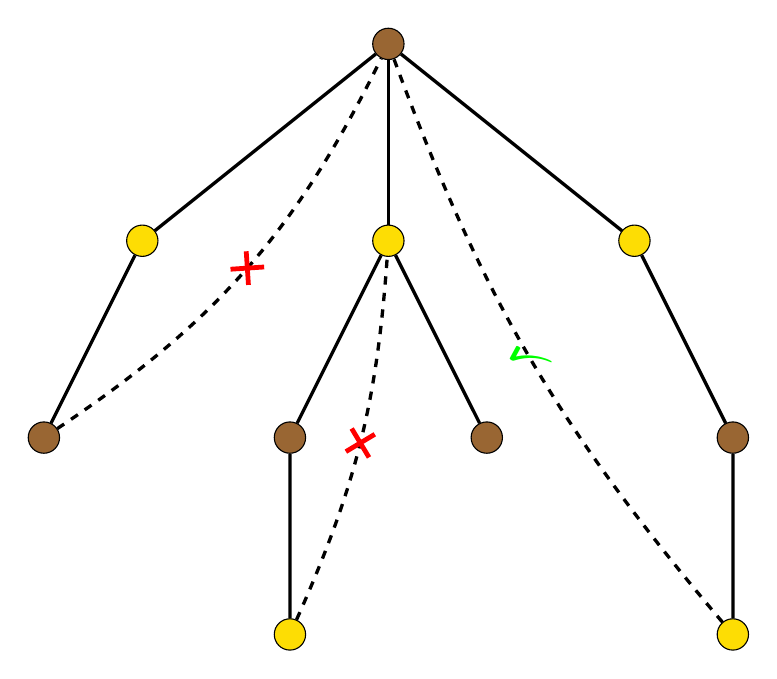
\begin{tikzpicture}[
    scale=2.5, 
    every node/.style={draw,circle,inner sep=4pt}
]

\begin{scope}
    % vertices.
    \node [fill=brown!80!black]   (1) at (0,0) {};
    \node [fill=yellow!80!orange] (2) at (-1.25,-1) {};
    \node [fill=yellow!80!orange] (3) at (0,-1) {};
    \node [fill=yellow!80!orange] (4) at (1.25,-1) {};
    \node [fill=brown!80!black]   (5) at (-1.75,-2) {};
    \node [fill=brown!80!black]   (6) at (-0.5,-2) {};
    \node [fill=brown!80!black]   (7) at (0.5,-2) {};
    \node [fill=brown!80!black]   (8) at (1.75,-2) {};
    \node [fill=yellow!80!orange] (9) at (-0.5,-3) {};
    \node [fill=yellow!80!orange] (0) at (1.75,-3) {};
    % tree edges.
    \draw [very thick] (1) -- (2);
    \draw [very thick] (1) -- (3);
    \draw [very thick] (1) -- (4);
    \draw [very thick] (2) -- (5);
    \draw [very thick] (3) -- (6);
    \draw [very thick] (3) -- (7);
    \draw [very thick] (4) -- (8);
    \draw [very thick] (6) -- (9);
    \draw [very thick] (8) -- (0);
    % other edges.
    \draw [very thick,dashed,bend right=15] (5) to node [draw=none,pos=0.5,sloped] {\Cross} (1);
    \draw [very thick,dashed,bend right=10] (9) to node [draw=none,pos=0.5,sloped] {\Cross} (3);
    \draw [very thick,dashed,bend left=10] (0) to node [draw=none,pos=0.5,sloped] {\Checkmark} (1);
\end{scope}

\end{tikzpicture}

\end{document}
